
\documentclass{sig-alternate-05-2015}

% The following \documentclass options may be useful:

% preprint      Remove this option only once the paper is in final form.
% 10pt          To set in 10-point type instead of 9-point.
% 11pt          To set in 11-point type instead of 9-point.
% authoryear    To obtain author/year citation style instead of numeric.

\usepackage{amsmath}
\usepackage{url}
\usepackage{subfigure}
\usepackage{listings}
\usepackage{eqnarray}

\usepackage{graphicx}
\usepackage{algorithm}
%\usepackage{algorithmic}
\usepackage{algpseudocode}% http://ctan.org/pkg/algorithmicx
\usepackage{amsmath}
\usepackage{mathtools}
\usepackage{caption}
\usepackage{diagbox}

\graphicspath{{./Figures/}}

\algdef{SE}[DOWHILE]{Do}{doWhile}{\algorithmicdo}[1]{\algorithmicwhile\ #1}

\begin{document}

\setcopyright{acmcopyright}

\conferenceinfo{XXXX 'XX}{Month d--d, 20yy, City, ST, Country}
\acmPrice{\$15.00}

% Uncomment one of the following two, if you are not going for the
% traditional copyright transfer agreement.

%\exclusivelicense                % ACM gets exclusive license to publish,
                                  % you retain copyright

%\permissiontopublish             % ACM gets nonexclusive license to publish
                                  % (paid open-access papers,
                                  % short abstracts)

%\titlebanner{}        % These are ignored unless
%\preprintfooter{}   % 'preprint' option specified.

\title{Demystifying Microarchitecture in GPU to Tune SGEMM Performance}
\subtitle{}


\maketitle

\begin{abstract}
In this paper, we present a thorough experience on tuning single precision general matrix multiplication(SGEMM)
in assembly level on Kepler GK110 architecture. First, we propose a methodology to demistify GPU's
microarchitecture-level optimizations. Based on the our own assembler KeplerAs, we debunk the
mystery of three performance-critical factors of microarchitecture,
which are control code pattern, register bank mapping and instruction throughput. Second, we tune
SGEMM performance by applying a comprehensive optimization which is never done in either CUDA or
PTX. The optimization strategies go through the architecture hierarchy including maximizing FFMA
throughput (core), eliminating register bank conflict (register), reducing global memory
transactions (shared memory), selecting data path to global memory (off-chip memory).
The optimized SGEMM TN, NN achieve an maximal floating-point efficiency of $88\%$ and $83\%$, which are $25\%$ and
$12\%$ higher than Cublas's $63\%$ and $71\%$ respectively.
This work will facilitate performance tuning of other core kernels on GPUs.
\end{abstract}

%\category{CR-number}{subcategory}{third-level}

% general terms are not compulsory anymore,
% you may leave them out
%\terms
%term1, term2

\keywords
SGEMM, Assembler, GPU, Performance

\section{Introduction}
Single Precision General Matrix Multiply (SGEMM) performs a multiplication of two single-precision matrices and is implemented as a basic routine of Level-3 in BLAS library~\cite{}. It has been extensively used in many scientific and engineering computing applications. Recently, SGEMM has drawn more and more effort on performance tuning since it is the performance critical kernel in deep learning applications~\cite{}.

As GPU provides more peak FLOP/S over CPU contemporarily, people tend to adopt GPUs to accelerate their floating-points intensive applications. In fact, SGEMM's performance highly relies on low level microarchitecture features. Hardware vendors also provide BLAS libraries tuned on their own processors, i.e. MKL/ACML for multicore x86 CPUs, CUBLAS/CLMath for GPUs. However, we always witness improvement of the third-party tuned implementations over these vendors' libraries. For multicore CPUs, based on the hand tuned assembly codes, OpenBLAS~\cite{} achieves the best performance in most cases. Although there is lack of an OpenBLAS-like library on GPUs, we observe that several on-going efforts~\cite{} achieve better performance than CUBLAS for either SGEMM or DGEMM by tuning assembly codes, too. Figure~\ref{} compares the maximal floating-point efficiencies achieved by SGEMMs in CUBLAS and third-party implementations. The third-parties improve performance by $xx\%$, $xx\%$ and $xx\%$ on G80, Fermi and Maxwell CUDA architectures, respectively. Unfortunately, there is no such a performance tuning work for SGEMM on Kepler architecture, which is the most popular architecture in current Tesla GPUs market. This work attempts to explore improvement space of floating-point efficiency of SGEMM on Kepler GPU.

However, there remain two issues to be addressed for accomplishing the microarchitecture based performance tuning on each generation of GPUs.
\begin{itemize}
\item {\em There is lack of a toolchain to identify GPU microarchitecture features and guide performance tuning.} Unlike general-purpose CPU community where a series of toolchains are available to tune performance in a bare metal way, only is the abstract model CUDA is encouraged. A major reason is the significant changes of each generation of GPU architecture. For example, the recent ISA is totally different from that of the first generation of GPU. The ISA is evolving to the trend where the graphics features are becoming less and less. Other microarchitectural details like register bank conflict and floating-point instructions dual issue are also different between two generations of GPUs. Fortunately, people have made some initial progress on such performance tuning tools due to the pursuit of extreme performance. These efforts are involved with either benchmarking~\cite{} or disassembler~\cite{} on a specific GPU architecture. We attempt to develop a methodology that provides a systematic way to identify microarchitecture by benchmarking, automatically decode instruction formats and generate ISA-compatible executable codes.

\item {\em There is lack of a comprehensive understanding of SGEMM's performance in terms of low level GPU microarchitecture.} Due to the lack of bare-metal tools on GPUs, most of SGEMM analysis are circumscribed at the levels of either CUDA  or PTX. Unfortunately, these analysis cannot directly diagnose neither compiler deficiency nor hardware defect. In fact, by observing the disassembled code of SGEMM in CUDA, we find that the generated control code is
very inefficient in exploiting FFMA dual issue. This means NVCC generated code does not
utilize shared $64$ cores on $192$ core SM, leaving them idle at most of time. A side effect of the limitation leads to a bias estimation of performance bound. We present a thorough analysis of performance which goes through the whole architecture hierarchy including instruction throughput, register allocation, shared memory transactions and global memory. The understanding of microarchitecture optimization help build a robust performance model of SGEMM.


\end{itemize}

In this paper we crack instruction encoding by performing a tough reverse engineering work, and build assembler to generate CUDA binary file for ISA-compatible assembly codes. Basically, due to the compatible grammar with CUDA {\tt cuobjdump}, we use CUDA toolchains to compile CUDA codes to {\tt cubin} file and then disassemble it to generate assembly codes. This approach supports users to optimize any code segment on the base of generated code instead of coding from scratch. By using this assembler, we design a set of microbenchmarks that demystify lots of GPU microarchitecture details such as instruction issue, warp schedule, register bank distribution and control code. It's helpful to understand and optimize performance of SGEMM. We apply a collection of optimizations to incrementally improve SGEMM performance one by one. More specifically, we make the following contributions:
\begin{itemize}
\item We propose an approach to reverse engineering approach to crack instruction encoding of GPU architecture, especially for control codes that orchestrate instruction scheduling. An assembler is developed to directly tune the assembly codes generated by CUDA compiler.
\item We design a bunch of benchmarks to reveal microarchitectural features which are undocumented by NVIDIA. They are important to understand and tune performance of GPU programs.
\item We implement the highest performance SGEMM routines on NVIDIA Kepler by applying the demystified microarchitecture-level optimizations. The achieved maximal floating-point efficiency is xx and xx on two GPUs, respectively.
\end{itemize}

Note that this work demonstrates the effectiveness on NVIDIA Kepler architecture. However, the approach is general for other NVDIA GPU architectures by minor  adjustments of instruction solver and benchmarking implementation. The demystified microarchitecture-specific optimizations are further applied performance tuning on other NVIDIA GPU architectures. The rest of this paper is organized as follows.

\section{Background}
Since we seek to establish an assembly-level optimization approach to SGEMM, this section introduces some CUDA binary utilities which are used in our work. Besides, we highlight the tunable factors that determine SGEMM performance on GPU architecture.

\subsection{CUDA Binary Utilities}
\label{sec:cuda}

A CUDA binary file is an ELF-formatted file generated by CUDA compiler {\tt nvcc}. It is also called {\em cubin} file, which can be either embedded into the host executable file or generated separately by using the "{\em -cubin}" option of {\tt nvcc}. In order to check {\em cubin} files, CUDA toolkit introduces three binary tools and documents on ISAs of several generations of GPUs from GT200 to Maxwell architecture. These binary tools only provide very limited functionalities to users. For instance, both {\tt cuobjdump} and {\tt nvdiasm} disassemble {\em cubin} files to {\em sass} ones, which are readable assembly codes for examining possible performance issues in GPU programs. For each instruction in the executable code sections, the tools list its address in hexadecimal, name in string and encoded number in hexadecimal. For example, an {\tt IADD} instruction might be printed as follows: \\\\
$/*0048*/~~~~IADD~~R0,~~R2,~~R0;~~~~/* 0x4800000000201c03 */$\\\\
Unfortunately, these tools do not enable us to directly modify the assembly codes for tuning performance. What we can do is to refine CUDA C codes after examining the read-only assembly codes iteratively. In fact, an assembler is required to manipulate assembly codes. Although NVIDIA doesn't release its internal assembler and instruction encoding format, the printed third field--encoded number, combining with the released ISA reference~\cite{}, provides clue to crack instruction format (in Section~\ref{sec:assembler}).


\subsection{Performance Factors of SGEMM }
It's well-known that the primary factors of SGEMM performance are the blocking parameters for exploiting data reuse through memory hierarchy. For an instance of GPU, they are shared memory blocking factor and register blocking factor. For the purpose of completeness, we describe a blocking algorithm which is similar with that in other literatures~\cite{magma}~\cite{nervana_sgemm_wiki}~\cite{lai}~\cite{tan}.

Algorithm~\ref{gemm} shows the skeleton of SGEMM blocking algorithm. Task partition is based on result matrix $C$.
Each thread block of $tx*ty$ threads is responsible to compute a $bm*bn$ block of submatrix $C$,
where $bm, bn$ is number of rows and columns of submatrix $C$, respectively.
In order to compute $bm*bn$ block of submatrix $C$, we need $bm*bk$ submatrix from A and $bk*bn$
sub-matrix from B.
In this way, $A$, $B$ and $C$ are divided into $M*K$, $K*N$ and $M*N$ grids of $bm*bk$, $bk*bn$ and $bm*bn$ blocks, respectively, where
$M=\Bigl\lfloor \frac{m+bm-1}{bm} \Bigr\rfloor$,
$K=\Bigl\lfloor \frac{k+bk-1}{bk} \Bigr\rfloor$,
$N=\Bigl\lfloor \frac{n+bn-1}{bn} \Bigr\rfloor$.

\begin{algorithm}
      \caption{SGEMM blocking algorithm}\label{gemm}
  \begin{algorithmic}[1]
      \State The size of thread block: $tx*ty$
      \State Register: accum[$rx*ry$], rA[$2*rx$], rB[$2*ry$]
      \State load one $bm*bk$ block of A into smA[$bk$][$bm$]
      \State load one $bk*bn$ block of B into smB[$bk$][$bn$]
      \Do
      \For {i = 1 to $bk$ } \Comment Unrolling for loop
      \State load one column of A in smA into rA[0 . . . $rx$]
      \State load one row of B in smB into rB[0 . . . $ry$]
      \State accum[0 . . . $rx$][0 . . .$ry$]+ = rA[0 . . . $rx$]* rB[0 . . . $ry$]
      \EndFor
      \State load one $bm*bk$ block of A into smA[$bk$][$bm$]
      \State load one $bk*bn$ block of B into smB[$bk$][$bn$]
      \State bar.sync
      \doWhile {pointer in B is out of range}
      \State merge accum[0 . . . $rx$][0 . . . $ry$] with $bm*bn$ block of C.
  \end{algorithmic}
\end{algorithm}

According to the blocking algorithm, SGEMM performance is affected by the hierachical memory blocking and unrolling factors in the inner loops. Table~\ref{tab:reg} estimates data movement volume through register, shared memory and global memory. The tuning of these factors is conducted in two folds which are memory bandwidth and latency. In fact, with the estimations in Table~\ref{tab:reg} it is relatively easy to tune proper parameters to eliminate bound of memory bandwidth~\cite{magma}~\cite{tan}. The difficulty is latency, which is closely related to specific microarchitecture such as instruction sequence, instruction type and so on. However, the microarchitectural optimizations depends on the availability of an assembler and deep understanding of microarchitectural features.

\begin{table}[!t]
\caption{Data movement volume in the blocking algorithm}
\centering
\scalebox{1.0} {
\begin{tabular}{|c||c|}
\hline
Data Path& Data Volume\\
\hline
global$\Rightarrow$regitster ({\tt LDG})& $\frac{bm*\times bk}{rx} + \frac{bn\times bk}{ry}$\\
\hline
register$\Rightarrow$shared ({\tt STS})& $\frac{bm\times bk}{rx} + \frac{bn\times bk}{ry}$\\
\hline
shared$\Rightarrow$register ({\tt LDS})& $bm\times bk + bn\times bk$\\
\hline
\end{tabular}
}
\label{tab:reg}
\end{table}

\section{Demystifying Microarchitecture Feature}
\label{sec:assembler}

\subsection{Methodology}
We propose a methodology to demystify GPU microarchitecture features and correlate them with performance. The workflow consists of three components.  The first one is CUDA binary tools, which are leveraged to generate assembly codes for sample programs or libraries. A sample program is synthetic CUDA file which is targeted to generate some specific instructions. A library might provide a high coverage of instruction sets. For example, the CUBLAS library contains almost all instructions used in SGEMM routine. As introduced in section~\ref{sec:cuda} these generated assembly files ({\em sass}) provide instruction encoded number to be cracked.

The instruction solver takes the assembly files as input to decode 64-bits binary representation of each instruction. We design a set of algorithms to solve all fields of the binary instruction. These fields include {\em register, predicate, address, immediate, constant} and {\em opcode}. The solver retrieves the undocumented ISA specification, which is used to implement an native assembler. Then, we design a rigorous microbenchmark and leverage the assembler to tune code at assembly language level. In the end, the tuning process will lead to some practical observations on the correlation between microarchitecture and performance.

\begin{figure}[htbp]
\begin{center}
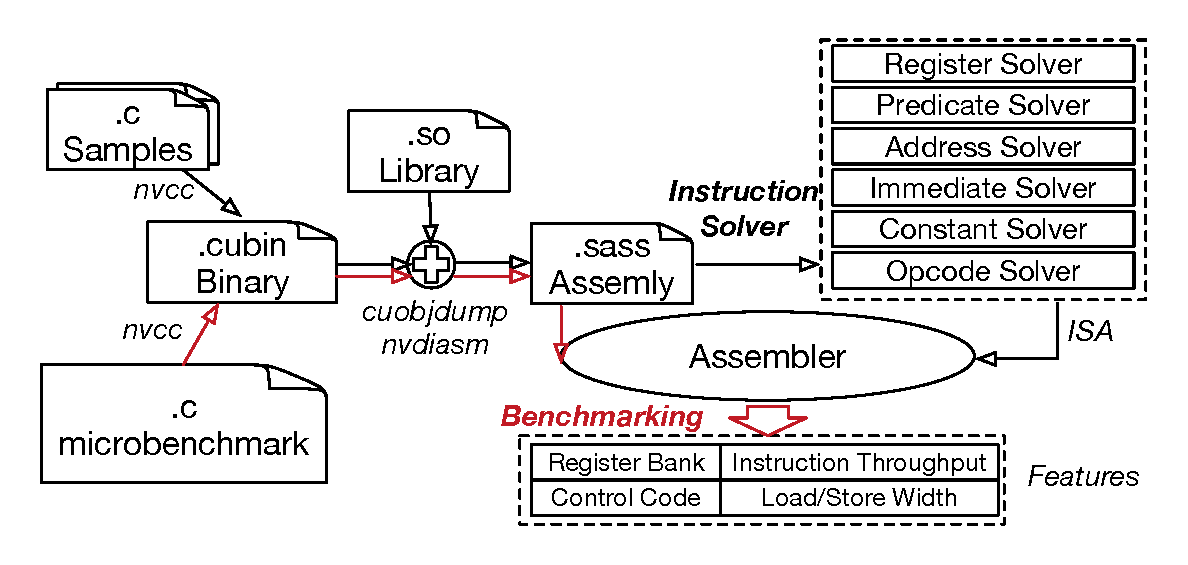
\includegraphics[scale=0.45]{methodology}
\caption{A schematic diagram of demystifying GPU microarchitecture features by leveraging CUDA binary tools. The back arrows represents the workflow of instruction solver while the red ones represents that of benchmarking to find out correlation between microarchitecture and performance.}
\label{fig:workflow}
\end{center}
\end{figure}

\subsection{Instruction Solver}
GPU instruction is composed of  serval fields: opcode, register, immediate, predicate register, modifiers. Encoding of some fields can be infered by their names, for example, R5's encoding could be 101, 0x9's encoding could be 1001. For this kind of fields, we could use similar method to determine their position and length. Encoding of some fields are mnemonic symbols, such as opcode, we can not infer encoding of FFMA by its name.
\subsubsection{Fixed Length Field}

\begin{algorithm}
      \caption{Solver}\label{integer_solver}
  \begin{algorithmic}[1]
      \State currpos=\{\}
      \State prepos=\{0,1,2,...63\}
      \State input: instmap
      \State output: pos, length
      \While {lenght(currpos) != 1}
      \State inst=instmap[random()]
      \If {inst.src1type == immediate}
      \State instencode=inst->encode64bit
      \State immbin = completecode(imm)
      \State pos = 0
      \While {pos + length(immbin) < 64}
      \If {strcmp(immbin,instencode+pos,length(immbin)}
      \State pushback(currpos, pos)
      \EndIf
      \EndWhile
      \State currpos = intersect (curpos, prepos)
      \State prepos = currpos
      \State currpos=\{\}
      \EndIf
      \EndWhile
      \State return curpos[0]
  \end{algorithmic}
\end{algorithm}

For fields whose encoding can be infered by its name, such as immediate, register index, predicate register, address etc., we can use Algorithm~\ref{} to solve it.
First, we random pick instruction that have these fileds, express field in binary. Second, we match field binary in $64$
bit instruction, and find possible candidate. There may be more than one instructions. Third, we merge current candidate
with previous candidate, if length of candidate is $1$ and return, else set current candidate to previous candidate, current candidate to null, random pick next instruction. repeat second step.
\subsubsection{Variable Length Opcode}
Opcodes does not show their encoding literally. One possible way is to write instruction {\tt PTX} code with flags based on syntax on Nvidia
PTX manual, generate encoding by using NVDIA toolchain.
Then, We can find the minimum opcode by strip out operand mask. Flags can be found by strip out opcode and operand mask.
This method is fast, but due to the uncompleteness of Nvidia document, we can not find out all the opcode and
instruction flags.
Other method is using brute force to emulate possible binary combinations after striping out operand mask.
Normally, each instruction have $3$ operand, we have $64-8*3-4=36$ bits left to probe. We prunch the search space by
recognize possible position that represent opcode.  However, by random probling bit
by bit, we find opcode is at top $10$ bit and lower $2$ bit represent opcode and other bits represent flags. We only emulate these bit.
The space is acceptable. Then we find the minimal opcode without any flags. The method allow use to find instructions
that are not listed on NVIDIA document, such as {\tt ALD}.

\begin{algorithm}
      \caption{Solver}\label{opcode}
  \begin{algorithmic}[1]
      \State for each instruction in PTX generated database
      \For {i=0; i < num\_inst; i++} 
      \For {j=0; j < 64; j ++}
      \If {isoperand(encode[i][j] == 0) and encode[i][j]== 0}
      \State newcode = setbit(j, 1)
      \State newinst=nvdisasm(newcode)
      \If {sameop(newinst,oldinst) == 0 and isvalid(newinst) }
      \State pushback(j)
      \EndIf
      \EndIf
      \EndFor
      \EndFor
  \end{algorithmic}
\end{algorithm}

\begin{algorithm}
      \caption{minime opcode}\label{opcode}
  \begin{algorithmic}[1]
      \State generate all combinations
      \State group by opcode, then operand
      \State sort the 12 bit binary 
      \State find the value with minimze value
  \end{algorithmic}
\end{algorithm}

\subsubsection{Modifier}
Modifiers (also called flags) are complex than the above, because its position is spanned along the left bits and one instruction may have
more than one kinds of modifers, for example {\tt LD} has u8, u16, 32, 64, 128 width information and also CG, LU cache
information. By stricking out opcode and oprand mask, we have around $24$ bits left. Based on our observation, we find
default value for modifier is $0$, modifier only happen when at least one bit is set. We can find the modifier possible position
by greedily set the lefted bit one by one, the time complexity is O(24) instead of $O(2^{24})$. The bit is typically less
than $10$ bit. After finding the candidate, we enumerate these bit, and group each kind.

\begin{algorithm}
      \caption{Solver}\label{opcode}
  \begin{algorithmic}[1]
      \If {bit[i] == 0 and isop(bit[i] == 0) and isoprand(bit[i])}
      \State newcode = setbit(i, 1)
      \State newinst=nvdisasm(newcode)
      \If {sameop(newinst,oldinst) == 0 and isvalid(newinst) }
      \State pushback(i)
      \EndIf
      \EndIf
  \end{algorithmic}
\end{algorithm}

\begin{algorithm}
      \caption{findflagkind}\label{opcode}
  \begin{algorithmic}[1]
      \State sort each field alphabatly
      \For each kind 
      \State merge all positions
      \EndFor
  \end{algorithmic}
\end{algorithm}

\subsection{Correlating Microarchitecture with Performance}
With the assembler we tune the assembly codes of microbenchmark. According to the performance tuning results, we correlate microarchitecture with performance variants that guide performance optimizations in real applications. The correlation is presented as several meaningful observations, which are categorized into four microarchitectural features of {\tt control} function, {\tt register} allocation, {\tt arithmetic} throughput and {\tt memory} operation.

\begin{figure}[htbp]
\begin{center}
%\includegraphics[scale=1.0]{table}
\caption{Different control codes regulate {\tt FFMA} throughput.}
\label{fig:control}
\end{center}
\end{figure}

{\em {\bf Observation 1--[Control]}: The execution sequence of instructions is regulated by control codes. Both warp scheduling and issue mode are tunable by setting control codes.}

Starting with the Kepler architecture NVIDIA has been moving some control logic off of the chip and into kernel instructions which are determined by the assembler. This evolution provides programmer a chance to make globally optimal decisions on scheduling and other control aspects if an assembler is available. The disassembly code indicates that every 64 bits control code controls $7$ instructions. We identify that both higher $6$ bits and lower 2 bits are {\em opcode} of control code, and the middle 56 bits are used to control the execution of $7$ instructions, each of which is assigned $8$ control bits.

For the eight control bits, we identify their meanings by examining CUBLAS disassembly codes and tuning a {\tt FFMA} throughput microbhenchmark. We observe that the $7$th bit of the control code of {\tt TLD} instruction is $1$, which indicates a texture dependency barrier due to weak consistent memory model. It's verified that some illegal values are loaded if this bit is not set. Similarly, we discover that the $5$th bit means shared memory dependency barrier, the $4$th bit means global memory dependency barrier. Figure~\ref{} shows that {\tt FFMA} throughput varies with all control bit values from 0 to 255. As shown in this figure, the throughput linearly decreases with the increasing values represented by the $0-3$ bits. That implies that these $4$ bits set the number of stall cycles before issuing the instruction. Further, the microbenchmarking reveal some specific patterns of control codes:

\begin{itemize}
\item When the control bits are set to be $0x40$, the scheduler suspends a warp of the instructions for 32 cycles.
\item $0x04$ means dual issue mode. If two consecutive instructions is controlled by $0x04$ and $0x05$, the throughput can reach the maximum. Single issue control code is $0x00$.
\item $0x20|n$ means a warp is suspended for $n$ cycles before issuing the next instruction, where $n$ is number between 0 and 15.
\end{itemize}


{\em {\bf Observation 2--[Register]}: Irrespective of single- or dual-issue mode, register bank conflict is only caused by source operands, and degrades instruction throughput by up to $17\%$.}

For CUDA programming model it is well-known that shared memory bank conflict is an important performance factor. In fact, recent researches~\cite{} noticed that register bank conflicts are nontrivial to performance.  In order to probe register bank conflict, our microbenchmark measures instruction throughput for different combination of {\tt FFMA} register operands. Table~\ref{tab:th} shows an example of the combination which results in variance of efficiency. The numbers in the fifth column represent the number of registers conflict in the same bank. This experiment is conducted in single-issue mode by setting control code to be $0x20$. The theoretical efficiency is $128/192=66.67\%$. In fact, we observe that both single- and dual-issue mode produce the same variance of instruction throughput. Besides, from the experimental results we observe that:
\begin{itemize}
\item Destination operand will not contribute to bank conflict, no matter which bank is assigned to it.
\item When source operands have 2-way conflict, the throughput will drop by 2.33\% in single issue
    mode. When source operands have 3-way conflicts, the throughput will drop by 17.17\%.

 \item On Kepler architecture, our microbenchmark finds out a proper distribution of registers for eliminating bank conflict. The distribution is summarized in Table~\ref{tab:reg}, which confirms the follow the rule~\cite{}: \\
 bank0$\Leftarrow$($Rindex \% 8 < 4$ \&\& $Rindex \% 2 == 0$) \\
 bank2$\Leftarrow$($Rindex \% 8 < 4$ \&\&
$Rindex \% 2 == 1$) \\
bank1$\Leftarrow$($Rindex \% 8 > 4$ \&\& $Rindex \%2 == 0$) \\
bank3$\Leftarrow$($Rindex \% 8 < 4$ \&\&
$Rindex\% 2 == 1$)\\
where $Rindex$ is the register number. This rule will guide the performance tuning in the following SGEMM implementation.

\end{itemize}

\begin{table}[htbp]
\caption{The efficiency of instruction throughput varies with difference register bank distribution. {\it Inst} : instruction pattern, {\it Th/SM}: the instruction throughput per SM, {\it Eff}: efficiency of throughput.}
\centering
\scalebox{1.0} {
\begin{tabular}{|c||c|c|c|}
\hline
Inst &Th/SM&Eff&Conflicts \\
\hline
{\tt FFMA R5,R4,R1,R0}&127.50&66.40\%&0\\
\hline
{\tt FFMA R2,R4,R1,R0}&127.50&66.40\%&0\\
\hline
{\tt FFMA R5,R2,R1,R0}&119.18&62.07\%&2\\
\hline
{\tt FFMA R3,R2,R1,R0}&119.18&62.07\%&2\\
\hline
{\tt FFMA R5,R9,R3,R1}&94.52&49.23\%&3\\
\hline
{\tt FFMA R11,R9,R3,R1}&94.52&49.23\%&3\\
\hline
{\tt FMUL R4,R1,R0}&127.50&66.40\%&0\\
\hline
{\tt FMUL R4,R2,R0}&119.17&62.06\%&2\\
\hline
\end{tabular}
}
\label{tab:th}
\end{table}


\begin{table}[htbp]
\caption{Register distribution for zero bank conflict.}
\centering
\scalebox{1.0} {
\begin{tabular}{|c||c|c|c|c|c|c|c|c|c|}
\hline
Bank0&0&2&8&10&16&18&24&26&... \\
\hline
Bank1&1&3&9&11&17&19&25&27&... \\
\hline
Bank2&4&6&12&14&20&22&28&30&... \\
\hline
Bank3&5&7&13&15&21&23&29&31&...\\
\hline
\end{tabular}
}
\label{tab:reg}
\end{table}

{\em {\bf Observation 3--[Arithmetic]}: With a proper control code and register allocation, {\tt FFMA} instruction throughput can approach the theoretical peak in dual issue mode.}

It's very intricate to tune instruction execution to improve instruction throughput. The previous work report a maximal throughput of {\tt FFMA} on a SM is $132$, which is much less than the theoretical throughput $192$ on Kepler. Our microbenchmarks reveal several key points of optimization to approach theoretical peak on Kepler. First, the control code must be set properly to dual issue adjacent instructions. Second, the ratio and interval of dual issue {\tt FFMA} instructions must be tuned into a specific pattern. Since each warp of extra computing unit is shared among two warps, when all threads are trying to fully dual issue every two adjacent {\tt FFMA}s, half of the scheduler would stall due to computing resource conflict. The ratio of dual issue and single issue should be $2:2$, and with a proper phase shift among two warp's executing pace, they could get access to the shared computing unit in turn. Third, the first instruction of the core loop needs to be aligned. This restriction is caused by the aligned position of control code in the instruction sequence. Last, {\tt FFMA} dual issue requires 6 register banks. Instruction order has to be adjusted to fully use Kepler's operand collector mechanism to avoid register bank conflicts. As shown in Table~\ref{tab:ffma}, these optimizations together improve {\tt FFMA}'s throughput  to be $190$, which is very close to the theoretical peak $192$.

\begin{table}[htbp]
\caption{Floating-point instruction throughput on Kepler}
\centering
\scalebox{1.} {
\begin{tabular}{|c||c|c|c|}
\hline
Inst name&operation&single issue&dual issue\\
\hline
{\tt FFMA} &c=a*b+c&127.52&190.35 \\
\hline
{\tt FMUL} &c=a*b&127.52&190.35 \\
\hline
{\tt FADD} &c=a+b&127.52&192\\
\hline
\end{tabular}
}
\label{tab:ffma}
\end{table}


{\em {\bf Observation 4--[Memory]}: For achieving higher memory bandwidth, shared memory prefers to 64-bits load instruction {\tt LDS.64} while global memory prefers to 128-bits load instruction {\tt LDG.E.128} with texture path.}

For the GPU memory hierarchy we focus on the programmer controllable memory resources--shared memory and global memory. On NVIDIA GPU architecture, there are different memory access widths (i.e., 32-bits,64-bits,128-bits) and paths (i.e., normal cache or texture cache). In fact, both NVIDIA document and previous works~\cite{} pointed out that wider instructions have longer pipeline latencies, which are also measured in our microbenchmark. In addition, we identify several bandwidth issues for memory optimization.

Intuitively, a wider load operation achieves higher bandwidth. We benchmark bandwidth of shared memory operations {\tt LDS} with different widths, i.e., {\tt LDS.32}, {\tt LDS.64}
and {\tt LDS.128}. The operations are specially arranged so that no shared memory bank conflict occurs in a warp. In the experiment, the amount of data are projected to the number of load instructions. For exmaple, if the data are loaded by $N$ {\tt LDS.128} instructions, then either $2N$ {\tt LDS.64} or $2N$ {\tt LDS.64} instructions are required. Figure~\ref{} compares the sequential memory access bandwidth with increasing volume of data. As shown in the figure, {\tt LDS.64} achieves the highest bandwidth $113GB/s$, which is about $60\%$ of the peak bandwidth\footnote{The theoretical shared memory bandwidth for each SM can be calculated as $Bandwidth=f_{core}*Width*Warpsize$ in
bytes, where $f_{core}$ is frequency of CUDA core, $Width$ is bank width, $Warpsize$ is warp size.}.

\begin{figure}[htbp]
\begin{center}
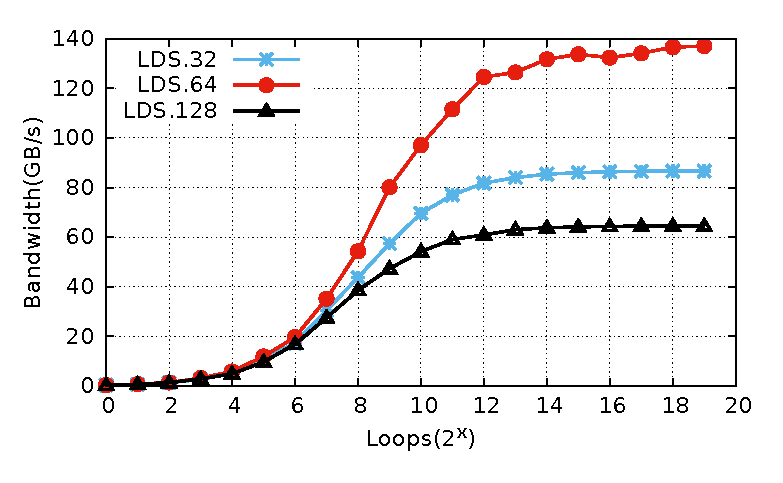
\includegraphics[scale=0.6]{lds_bandwidth}
    \caption{ Bandwidth of {\tt LDS.32}, {\tt LDS.64} and {\tt LDS.128}}
\label{fig:lds_bw}
\end{center}
\end{figure}

\begin{figure}[htbp]
\begin{center}
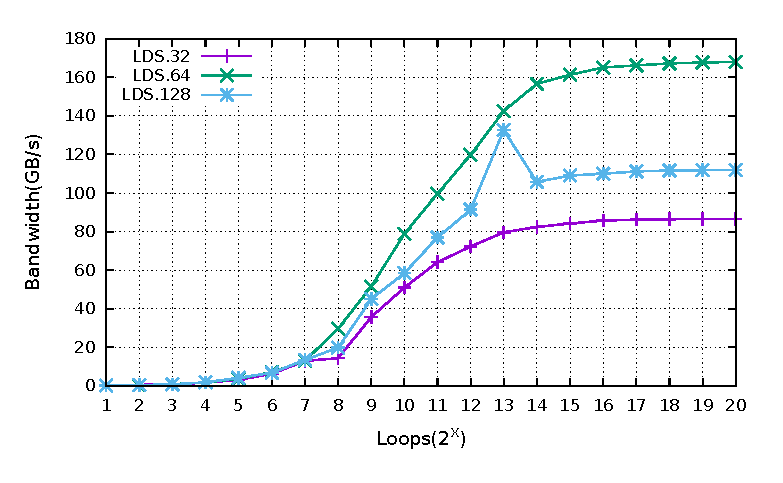
\includegraphics[scale=0.6]{lds_broadcast_bandwidth}
    \caption{ Broadcast bandwidth of {\tt LDS.32}, {\tt LDS.64} and {\tt LDS.128}}
\label{fig:lds_brd_bw}
\end{center}
\end{figure}

% global memory
There are two paths to global memory. One is from global memory to normal cache (L1 or L2), which is executed by {\tt LD} instruction. The other one is from global memory to texture cache, which is executed by {\tt LDG} instruction. Our microbenchmark launches $26$ thread blocks with $512$ threads, and specifies that each thread access $4$ words with a stride of $4*blockDim.x*gridDim.x$. As shown in  Figure~\ref{}, {\tt LDG} achieves higher bandwidth than {\tt LD}.


\section{Applying Optimizations to SGEMM }
\label{sec:optimization}
The demystified GPU microarchitecture features provides additional space to tune performance-critical kernels. We apply a series of incremental optimizations to improve SGEMM efficiency on Kepler architecture. The optimization strategies go through architectural hierarchy from core and register to memory. All the optimization strategies are inspired by our microbenchmark's observations.
\begin{itemize}
\item At core level, we orchestrate {\tt FFMA} instruction executions by a more efficient instruction scheduling pattern with respect to the proper control code.
\item At register level, we meticulously map operands to registers so that  bank conflicts are avoided in the inner loop iteration.
\item At memory level, we select appropriate shared memory load/store width and global memory data path to mitigate latencies.
\end{itemize}

\subsection{Instruction Scheduling}
It's ideal to keep warp scheduler dual issue instructions (i.e., {\tt FFMA}) all the time. However, for each SM on Kepler architecture, 64 cores share $4$ schedulers, each of which issues instructions to 32 cores as a warp. As noted in {\em observation 3}, the best pattern of {\tt FFMA} instructions block is a sequence of 2 dual issues (4 {\tt FFMA}s) and 2 single issues ((2 {\tt FFMA}s)). As shown in Figure~\ref{}, the instructions in lines 2-3 and lines 6-7 are respectively grouped as two dual-issues. The other two instructions in line 10 and line 13 are two single issues in terms of floating-point instruction execution. As a comparison, most of the {\tt FFMA}s are single-issues in the CUDA compiler generated codes.


\begin{algorithm}
      \caption{NVCC generated assembly code}\label{nvcc}
  \begin{algorithmic}[1]
      \footnotesize
        \State /*0x08dc109c14801410*/
        \State [
        \State /*0348*/ FFMA R28, R41, R15, R28; /*0xcc007000079ca472*/
        \State /*0350*/ LDS.128 R12, [0x40];     /*0x7a700000201ffc32*/
        \State ]
        \State /*0358*/ FFMA R39, R41, R9, R39; /*0xcc009c00049ca49e*/
        \State /*0360*/ FFMA R29, R41, R10, R29; /*0xcc007400051ca476*/
        \State /*0368*/ FFMA R32, R41, R11, R32; /*0xcc008000059ca482*/
        \State [
        \State /*0370*/ LDS.128 R8, [0x50]; /*0x7a700000281ffc22*/
        \State /*0378*/ IADD R4.CC, R4, R21; /*0xe08400000a9c1012*/
    \State ]
  \end{algorithmic}
\end{algorithm}



\begin{algorithm}
      \caption{The optimized assembly code }\label{nvcc}
  \begin{algorithmic}[1]
      \footnotesize
        \State [
        \State -:-:D:-:04      FFMA R27, R150, R146, R27;
        \State -:-:D:-:05      FFMA R6, R149, R146, R6;
        \State ]
        \State [
        \State -:-:D:-:04      FFMA R7, R148, R147, R7;
        \State -:-:D:-:05      FFMA R2, R149, R147, R2;
        \State ]
        \State [
        \State -:-:D:-:04      FFMA R3, R148, R146, R3;
        \State -:-:-:-:00      LDS.64 R168, [R222+0x400];
        \State ]
        \State -:-:D:-:05      FFMA R9, R148, R152, R9;

        \State ]
  \end{algorithmic}
\end{algorithm}

\begin{figure}[htbp]
\begin{center}
%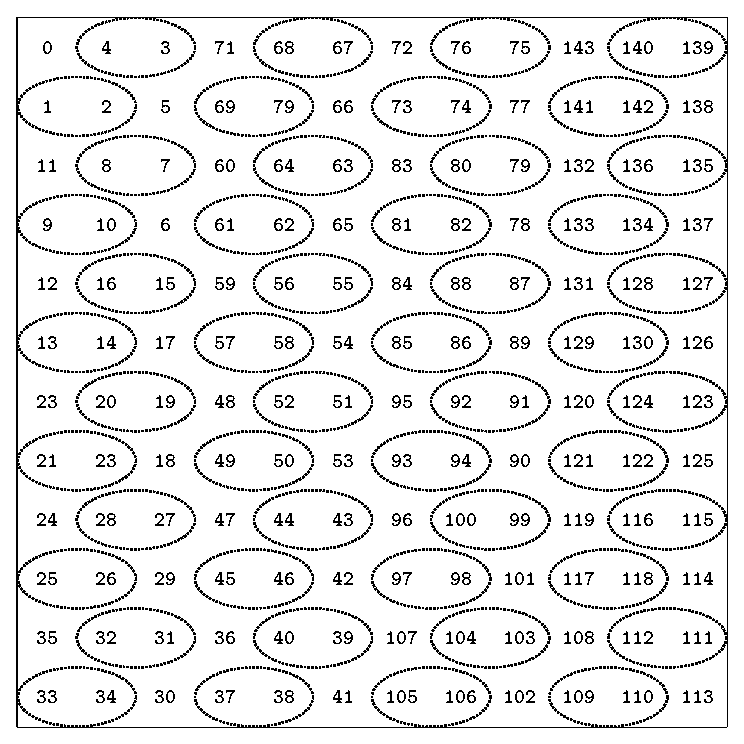
\includegraphics[scale=0.5]{order}
\caption{{\tt FFMA}s instructions scheduling for calculating a $8\times 8$ subblock of matrix C.}
\label{fig:order}
\end{center}
\end{figure}

Based on the basic {\tt FFMA} instruction block, the scheduling pattern is depicted in Figure~\ref{}, which illustrates the order of 144 {\tt FFMA}s instruction execution for calculating a $12\times 12$ subblock of matrix C. For example, the {\tt FFMA} to calculate $c_{00}$ is the first instruction to be issued. Then, both {\tt FFMA}s to calculate $c_{10}$ and  $c_{11}$ are simultaneously issued. We arrange all the {\tt FFMA} operations according to issue order illustrated in Figure~\ref{}.

Another advantage of this execution order is less register pressure due to register data reuse, which can facilitate operand collector mechanism~\cite{}. Operand collector is storage element coupled from register file and provides inputs to the data path of the processor core for executing an instruction. Operands may be cached and reused in the subsequent instructions. The assembly code in Algorithm~\ref{} lists the instructions to calculate $C_{22}, C_{21}, C_{30}, C_{31}, C_{20}, C_{40}$, where are corresponding to the orders of $7,8,9,10,11,12$ in Figure~\ref{}. The reuse happens as follows. The {\tt FFMA} in line 2 uses the cached operand {\tt R150} from the previous instruction block. Line 3 uses the cached operand {\tt R146} from the previous instruction. Similarly, The {\tt FFMA} in line 7 reuses the cached operands of   {\tt R149} and {\tt R147} from the previous two instructions, respectively.


After setting the order of {\tt FFMA}, other {\tt non-FFMA} instructions should be inserted in proper positions to assure
corretness of the program without losing performance. In order to tolerate instruction latency, we need to keep distance of dependent instructions to be larger than the latency. The distance can be approximately computed as
\begin{displaymath}
distance = \frac{4\times\#instructions}{7}
\end{displaymath}
In a schedule block, there are $7$ instructions which cost $4$ clocks to be issued in dual issue mode. In other word, if we want to have interleave
two instructions of $L$ distance, then $\frac{L*7}{4}$ instructions are needed. Besides, the remained number of slots to insert these instructions is estimated as follows:

\begin{displaymath}
\#slots = \frac{bm\times bn\times unroll}{ffmas\_in\_schedule\_block}=\frac{12\times 12\times 4}{6}=24\times 4
\end{displaymath}

According to these principles, we first arrange {\tt LDS}, {\tt STS}, {\tt LDG} due to their long latencies. The schedule slots are illustrated in two dimension as shown in Table~\ref{}.
Note that we use double buffers to hide latency of {\tt LDG} from global memory, which costs $200$ clock cycles.
Every $4$ loop requires $2$ {\tt LDG}s to load data from global memory to registers, $4$ {\tt STS}s to store data from registers to shared memory. There is a read after write (RAW) dependency between {\tt
LDG} and {\tt STS}. The simple model estimates that $\frac{200\times 7}{4} = 350$ are needed instructions between them. As shown in Table~\ref{}, we put {\tt LDG} and  {\tt STS} in position $P[77][3]$ and position $P[65][2]$, respectively. Thus, the number of instructions between them are $143-77 + 144\times 2 +
65=419$, resulting in a distance of $\frac{4\times 419}{7}=239$ clocks, which is enough to hide latency of {\tt LDG}s.

The arrangement of {\tt LDS}s, which load data from shared memory for double buffers of both $A$ and $B$, follows the same way with {\tt LDG}s.
A {\tt LDS} has a latency of $40$ clock cycles, $\frac{40\times 7}{4}=70$ instructions are needed to interleave {\tt LDS} and {\tt
FFMA}. As shown in Table~\ref{}, {\tt LDS} in $P[11][3]$ read data from {\tt STS} in position $P[65][2]$, the distance is more than $40$ clock
cycles. In the end, a {\tt BAR.SYNC} should be inserted after {\tt STS} before {\tt LDS} to make sure that data in shared memory is ready. Other instructions like {\tt XOR},
{\tt IADD}, {\tt ISETP} are inserted according to data dependency, there is almost no performance loss due to little latency.

\begin{table}[!t]
\caption{The position table of {\tt Non-FFMA} instructions. The inner-loop is unrolled by 4 times. The first column records slot numbers.}
\label{tab:position}
\captionsetup{font=scriptsize}
\centering
\scalebox{0.78} {
\begin{tabular}{|c|c|c|c|c|}
\hline
\diagbox[width=4em, height=3em]{slot}{unroll} & 0 &1 &2 &3 \\
    \hline
    5 & ISET P0 & IADD trackA0 & & XOR readBs \\
    \hline
    11 & LDS.64 readAs & LDS.64 readAs & LDS.64 readAs & LDS.64 readAs \\
    \hline
    17 & LDS.64 readAs & LDS.64 readAs & LDS.64 readAs & LDS.64 readAs \\
    \hline
    23 & LDS.64 readAs & LDS.64 readAs & LDS.64 readAs & LDS.64 readAs \\
    \hline
    29 & LDS.64 readAs & LDS.64 readAs & LDS.64 readAs & LDS.64 readAs \\
    \hline
    35& IADD K, -4 & IADD trackA1 & TEXDEPBAR & \\
    \hline
    41 & LDS.64 readBs & LDS.64 readBs & LDS.64 readBs & LDS.64 readBs \\
    \hline
    47 & LDS.64 readBs & LDS.64 readBs & LDS.64 readBs & LDS.64 readBs \\
    \hline
    53 & LDS.64 readBs & LDS.64 readBs & LDS.64 readBs & LDS.64 readBs \\
    \hline
    59 & LDS.64 readBs & LDS.64 readBs & LDS.64 readBs & LDS.64 readBs \\
    \hline
    65 & & &STS.64 writeS & ISETP P2 \\
    \hline
    71 & & & & \\
    \hline
    77 & & IADD trackB0 & & LDG trackA \\
    \hline
    83 & LDS.64 readAs & LDS.64 readAs & LDS.64 readAs & LDS.64 readAs \\
    \hline
    89 &ISETP P3 & & &\\
    \hline
    95 & LDS.64 readAs & LDS.64 readAs & LDS.64 readAs & LDS.64 readAs \\
    \hline
    101 & & & STS.64 loadB0 & LDG trackB \\
    \hline
    107 & & & STS.64 loadB2 & XOR writeS \\
    \hline
    113 & & & & \\
    \hline
    119 & LDS.64 readBs & LDS.64 readBs & LDS.64 readBs & LDS.64 readBs \\
    \hline
    125 & & & XOR readAs & \\
    \hline
    131 & LDS.64 readBs & LDS.64 readBs & LDS.64 readBs & LDS.64 readBs \\
    \hline
    137 & & & & \\
    \hline
    143 & & IADD trackB1 & BAR.SYNC & BAR Loop \\
    \hline
\end{tabular}
}

\end{table}

\subsection{Register Allocation}

To allocate register for $A$ column, $B$ row and $C$ submatrix, we have three considerations: correctness, no bank
conflict and allocate register index tightly.
{\tt LDG.128} restricts $4$ words alignment restriction for register.
Nvidia GPU does not have $128$ bit register, in order to use $128$ bit load, one destination register $RN$ is given, result is writen to
$RN+1$, $RN+2$, $RN+3$. There is undocumented restriction: $N\%4==0$, otherwise illegal instruction error will be reported.
It's not hard to understand this restriction, $4$ words align for {\tt LDG.128} make hardware logic simpler saving die area.
Since we will use {\tt LDG.128} to load $A$ and $B$, there are $2$ bank allocation choices due to $N\%4==0$ restriction and
bank distribution of Kepler. We assume allocate $A$ matrix bank $\begin{bmatrix} 0 \\ 1  \end{bmatrix}$,
$B$ bank $\begin{bmatrix} 2 & 3 \end{bmatrix}$ as shown in Figure, we have 2 choices left for $C$.
$\begin{bmatrix} 1 & 2 \\ 3 & 0  \end{bmatrix}$
$\begin{bmatrix} 3 & 1 \\ 0 & 2  \end{bmatrix}$
We have $2i\times2$ bank patterns for SGEMM, we choose $\begin{bmatrix} 0 \\ 1  \end{bmatrix}$ $\begin{bmatrix} 2 & 3 \end{bmatrix}$
$\begin{bmatrix} 1 & 2 \\ 3 & 0  \end{bmatrix}$ for $A$, $B$ and $C$ respectively as shown in Figure.
To allocate actual register index, we choose continuous register index so that register index do not get too big to
exceed 255 restriction. From figure, we can verify that $C_{ij}$, $A_i$ and $B_j$ have different banks, for example
$C_{01}$'s color is white, $A_0$'s color is green and $B_1$'s color is red, hence no bank conflicts.

\begin{figure}[htbp]
\begin{center}
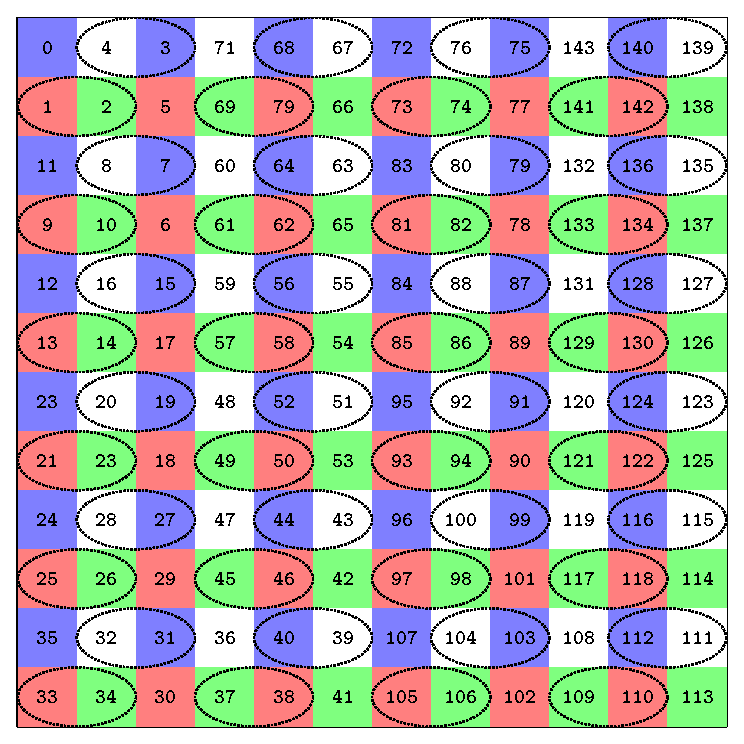
\includegraphics[scale=0.55]{reg}
\caption{Register bank allocation: number in the cell is register number. Double buffering column
    $A$ and row $B$. Leftest two columns are registers allocated to one column of $A$ sub-matrix, the
top two rows are registers allocated to one row of sub-matrix $B$, others are registers for
sub-matrix $C$. Green cells means bank0, blue cell means bank1, gray cell means bank2, red cell
means bank3.}
\label{fig:reg}
\end{center}
\end{figure}

\begin{figure}[htbp]
\begin{center}
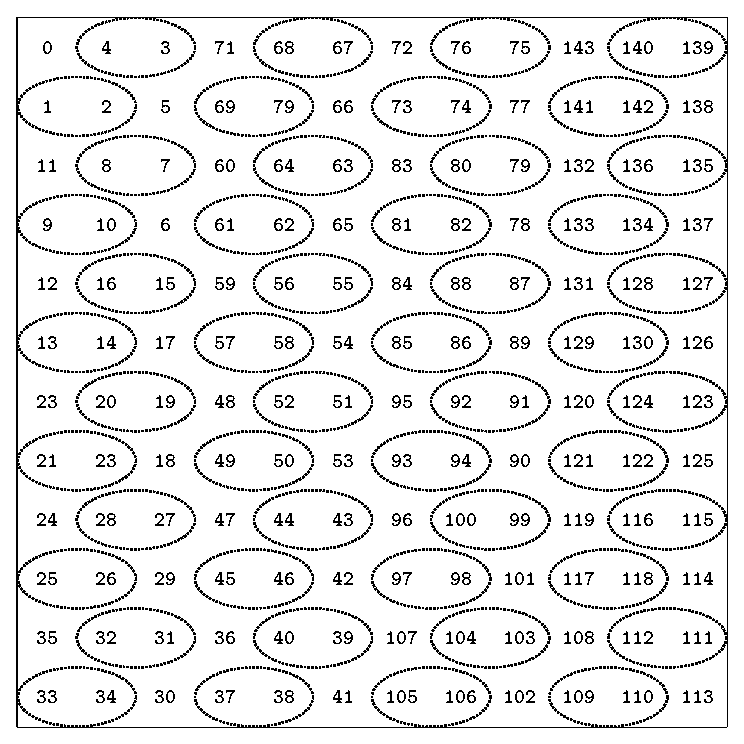
\includegraphics[scale=0.6]{order}
\caption{FFMA order: the numbers in the cells mean FFMA executing order, not register number.
Dashed ellipses across two cells mean two FFMA instructions are executed at same clock cycle. }
\label{fig:order}
\end{center}
\end{figure}

\subsection{Memory Movment}
According to the optimization observation on memory access suggested by microbenchmark, we use {\tt LDS.64} to load data from shared memory and {\tt LDG.E.128} to load data from global memory. Specifically we have additional reasons to adopt them in SGEMM kernel. First, the use of {\tt LDG.E.128} can reduce the number of {\tt non-FFMA} instructions. For example,  in the inner loop, the number of 32-bits load operations to read $A$ and $B$ is 12. The wider {\tt LDG.E.128} operation reduces the numbers to be 3. 

Second, it is another story for shared memory. The shared memory transaction size of 256 bytes forces that any shared memory request will be split into multiple transactions of 256 bytes. By inspecting the inner loop, we cannot control when the second transactions happen so that it is difficult to eliminate potential bank conflicts between {\tt LDS.128}s and {\tt FFMA}s. As for {\tt LDS.64}, it's determinable to avoid register bank since a transaction just happens at the position of {\tt LDS.64}. 



\section{Evaluation}

In this section, we compare the optimized SGEMM performance in Gflop/s with NVIDIA CUBLAS. The $12\sim 25\%$ improvement shows that the microarchitectural optimization makes sense of tuning SGEMM on GPUs.   We further present a quantitative analysis of the effect of each individual optimization strategy and an estimation of the upper bound performance.

The experiments are conducted on NVIDIA K20m GPU, which hardware configuration is summarized in Table~\ref{table:k20}. The compared CUBLAS is from CUDA $7.0$ version. In our experiments the sizes of matrix vary in $768\times768$, $1536\times1536$,$3072\times3072$,$6144\times6144$,$12288\times12288$.

\begin{table}[!t]
\caption{K20 Specification}
\centering
\scalebox{1.0} {
\begin{tabular}{|c||c|}
\hline
Metric& Value\\
\hline
SPs/SM &192\\
\hline
    SMs&13\\
\hline
Cores &2496\\
\hline
Frequency(MHz)&705\\
\hline
Memory Bus Width&320\\
\hline
Memory frequency&2600 Mhz\\
\hline
Bandwidth(GB/s)&208.0\\
\hline
Single FLOPS&3520\\
\hline
warp schedular per SM&4\\
\hline
dispatch unit/SM&8\\
\hline
Max registers/thread&256 \\
\hline
32-bit registers/SM&64K\\
\hline
LD/ST unit&32 \\
\hline
shared memory&48KB\\
\hline
L1 cache&16KB or 48KB\\
\hline
    L2 cache&1536KB\\
\hline
\end{tabular}
}
\label{table:k20}
\end{table}


\subsection{Overall Performance}
Figure~\ref{fig:sgemm_tn} reports the performance comparison of CUBLAS SGEMM and our optimized SGEMM.
Our SGEMM achieves $3104$ Gflop/s which efficiency is $3104/3520=88\%$. With the same matrix size, CUBLAS has $2216$ Gflop/s which efficiency is $63\%$. The comparison shows that our implementation achives 25\% performance improvement over CUBLAS. 

As the figure shows, the overall trend is that performance increases with bigger matrices. On one hand, the larger matrix size leads to a higher ratio of floating-point operations to memory operations, which is more close to the hardware arithmetic intensity. On the other hand, the larger matrix size increases occupation of the threading CUDA cores. The numbers of block ranges from $[768/192,768/192]=[4,4]$ to $[12288/192, 12288/192]$ $=[64,64]$. Since Kepler has $13$ SMs in total, matrix of size $768x768$ suffers from low utilization of massive cores. Therefore, we observe that there is significant growth in Gflop/s from 768 to 1536 for both ours and CUBLAS. With respect to the ratio of performance improvement, the optimization has less effect on the smaller matrix size than the larger one. The reason is that the performance is increasingly bounded by the microarchitecture rather than memory due to the higher arithmetic intensity. Thus, our microarchitecture-level optimization plays more important role on tuning performance.  

\begin{figure}[htbp]
\begin{center}
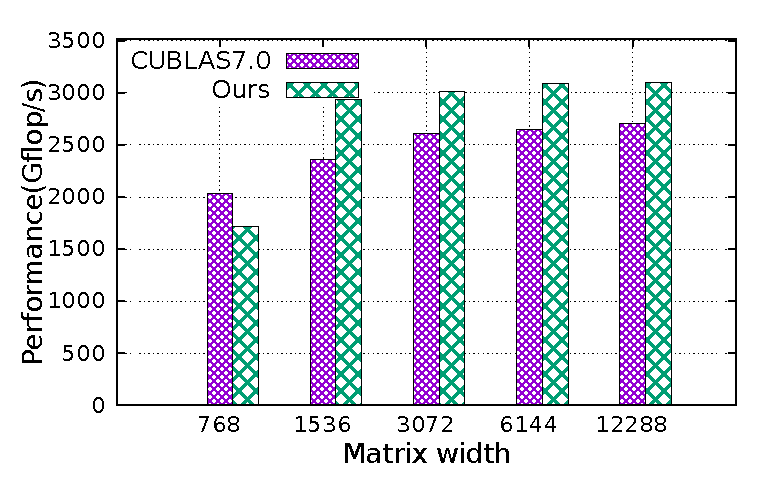
\includegraphics[scale=0.6]{sgemm_tn}
\caption{Performance comparison of CUBLAS and the optimized SGEMM }
\label{fig:sgemm_tn}
\end{center}
\end{figure}

\subsection{Performance Analysis}

\subsubsection{Profiling Microarchitectural Optimization}
In order to examine performance gain of different optimization strategies, we construct several intermediate implementations by incrementally applying the microarchitectural optimizations. 

{\it Baseline:}~~The baseline involves conventional optimizations including register blocking, global
memory double buffer, shared memory double buffer and unrolling, rather than assembly level optimization.
For example, baseline use default $32-bit$ {\tt LD} rather than $128-bit$ {\tt LDG} to load data from global memory.
Register allocation for $C$ is allocated orderly from $0$ to $143$, then $A$ and $B$ matrices. In this case, {\tt
FFMA}s will have $368/(144*4)=63.89\%$ and $64/(144*4)=11.11\%$ 3-way bank conflicts. Baseline does not apply dual
issue optimization either.

{\it +Reg:}~~The register allocation pattern described in section~\ref{} is applied to eliminate register bank conflict. No
instruction scheduling change between this version and baseline version.

{\it +LD128:}~~Use wider global load instruction.
Kepler has an L1 data cache, but it is designed for local rather than global memory access. So {\tt LD} will not be L1-cached, it may be L2-cached.

{\it +LDG128:}~~{\tt LD} is load instruction used in implementation. When {\tt LDG} is used, a {\tt TEXDEPBAR} is needed before using the data. 

{\it +InstSched:}~~Single issue is controlled by setting control code to $0x00$. Dual issue is fully enabled by utilizing the pattern described in section~\ref{}. For dual issue version, $NOP$ may be inserted for instruction alignment.

\begin{figure}[htbp]
\begin{center}
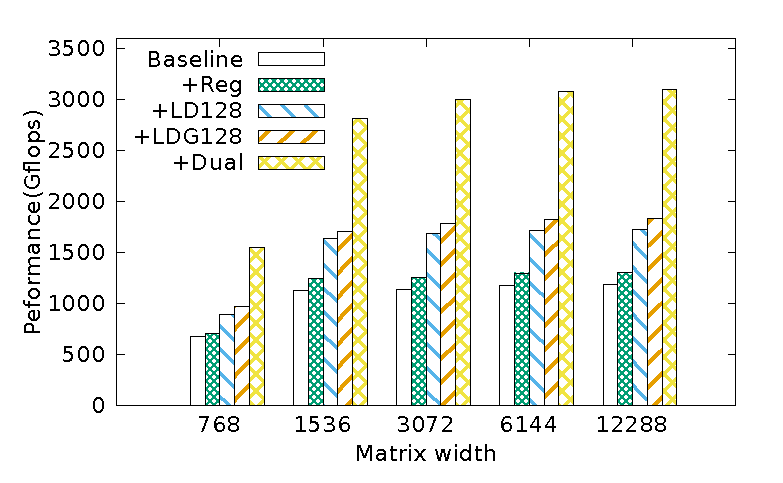
\includegraphics[scale=0.65]{tn_prof}
    \caption{Evaluation of each optimization method: {\tt conf} is register conflict, {\tt noconf} is no register bank conflict,
    {\tt single} is {\tt FFMA} single issue, {\tt LD} is using {\tt LD} as load instruction, {\tt LDG} is use {\tt LDG}
    as load instruction, 32-bit {\tt LD} instruction, {\tt dual} is {\tt FFMA} dual-issue.}
\label{fig:th_prof}
\end{center}
\end{figure}

Figure~\ref{fig:th_prof} illustrates performance gain of each optimization method.
As long as number of instructions is changed, instruction order needs reschedual to achive high peformance.
Compared with the baseline implementation, $2.6X$ speedups are gained by applying all the optimization.
Register bank conflict elimating imporves around $10\%$. wider load instruction improves $27\%\sim35\%$, texture cached
load instruction {\tt LDG} improves $5\%\sim12\%$. Dual issue improves the most, $84\%\sim106\%$. In most cases, the bigger matrix
size, the more improves except {\tt LDG} and {\tt LD}.

\subsubsection{Register Blocking Size Choosing}

Register blocking size is limited by instruction cache, shared memory size, registers per thread, the maximum number of threads in one block. 
In order to hide latency of shared memory, software pipelining using double
buffers is an efficient way. Each thread needs $rx\times ry$ registers to store result of $C$ submatrix, $rx$ and $ry$ to store a column of $A$
submatrix and a row of $B$ submatrix in current loop. In addition, the extra $rx$ and $ry$ registers are used for prefetching $A$ and $B$ from shared memory to
registers for next loop. Since the total number of registers should be less than $255$ in Kepler architecture, we have the following equations.
\begin{equation}
    rx\times ry + rx\times 2 + ry\times 2 < 255
\label{f_register}
\end{equation}
First, this function implies that the optimal solution should be in the case of $rx=ry$. Because the maximal number of register per thread is 255 and data load must be aligned with 128-bits, the blocking size might be $4\times 4$, $8\times 8$ and $12\times 12$. In fact, the blocking factor of $4\times 4$ leads to low data reuse in register files. Figure~\ref{fig:block} demonstrates $8\times8$ blocking and $12\times12$ blocking. $12\times12$ is better than
$8\times8$ in that, it has high computation memory ratio and higher instruction level parallelism. With respect to instruction scheduling optimization, $12\times12$ blocking has more slots to insert other {\tt non-FFMA} instructions, leaving more
space to schedule instructions, the overhead of {\tt LDS} can be amortized. Thus, the number of registers is $12*12+4*12=192$ used by both {\tt LD} and {\tt FFMA}, totally resulting $236$ registers with other address indices.The register number allows us to launch $256$ threads in a block. Each block of threads computes a $bm\times bn$ submatrix of $C$ by multiply $A_{bm,bk}$ and $B_{bk,
bn}$. 

\begin{figure}[htbp]
\begin{center}
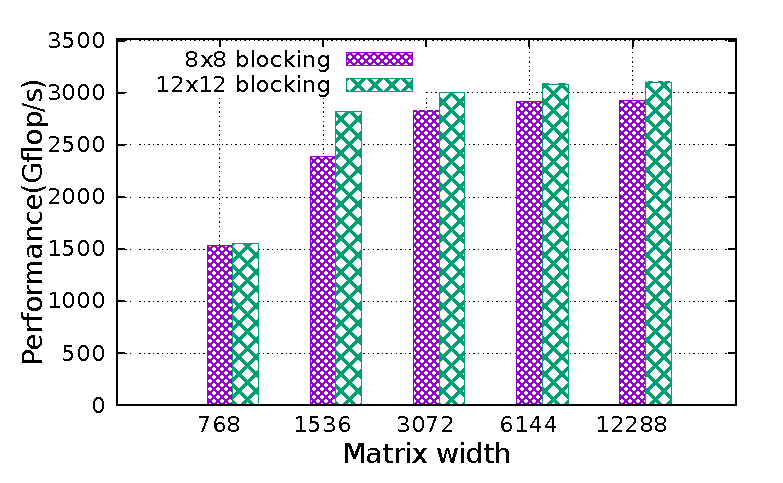
\includegraphics[scale=0.6]{block}
    \caption{Evaluation of different blocking size}
\label{fig:block}
\end{center}
\end{figure}

\subsubsection{Upper Bound Analysis}
We estimate the upper bound factors: {\tt LDS}, {\tt LDG} and {\tt FFMA}. They correspond to $3$ kinds of resources, shared
memory, global memory and computation power. In register blocking loop, each thread compute $bm*bn*bk$, read $bm*bk$
and $bn*bk$ words. The upper bound of global memory bandwidth can be modeled as:
\begin{displaymath}
    \frac{2*bm*bn*bk}{4*(bm*bk + bn*bk)} < \frac{Gflop/s}{bandwidth}
\end{displaymath}
According to parameters in our SGEMM implementation, $bm=bn=192$, $bk=4$, $Gflop/s=3520$, so $73$ GB/s is the minimal
requirement for global memory bandwidth in order to achieve peak $3520$ Gflops.
For shared memory, inside each loop, $(rx*bk + ry * bk)*tx*ty$ words will be read from shared memory, in which $tx$,
$ty$ is block dimension, $rx$, $ry$ is register blocking size. The computation is $bm*bn*bk$. Based on computation
shared memory ration,
\begin{displaymath}
    \frac{2*bm*bk*bn}{4*tx*ty*(rx*bk + ry *bk)}  = \frac{Gflop/s}{bandwidth}
\end{displaymath}

On Kepler GPU the minimum bandwidth requirement is $1173$GB/s, and for each SM of Kepler, bandwidth requirement is
$1173/13=90$ GB/s.
The hardware can provide $200$GB/s global memory bandwidth and $2349$GB/s shared memory bandwidth, which is
higher than requirement, and hence neither bandwidth of shared width nor global memory will be bottleneck.

The loss to peak performance can be explained as the following reasons. As we have shown in Section~\ref{sec:kepleras}, FFMA throughput can achieve $97.67\%$. The loss is about $2.33\%$, which may comes from overhead of warp scheduler in {\tt FFMA} dual issue mode. The double-buffering algorithm can amortize the latency of {\tt LDS}.
With $12x12$ register blocking and $4$ times unrolling, there will be $144*4=576$ {\tt FFMA} instructions in the loop.
With our designed {\tt FFMA} dual issue pattern, every $6$ {\tt FFMA} needs $4$ clock cycles in the pipeline.
It needs $4*144*4/6=384$ clock cycles for each thread,  two $128$ bits {\tt LDG} instruction are needed.
Each {\tt LDG} has $10$ clock penalty, the total {\tt LDG} penalty will be $2*10/384 = 5.2\%$. Other penalty comes from synchronization and writing $C$ matrix in the block.
%
% The following two commands are all you need in the
% initial runs of your .tex file to
% produce the bibliography for the citations in your paper.
\section{Related Work}
To our knowledge, this paper provides the first comprehensive study of demystifying NVIDIA GPU microarchitecture which is correlated with performance tuning in SGEMM. This section briefly discusses related work in assembler, microbenchmarking and SGEMM optimization.

The lack of assembler for public use motivates a series of work on developing toolchains to facilitate tuning codes in assembly level. For the early architecture G80, Decuda~\cite{decuda} demonstrated the feasibility to operate the limited number of assembly instructions. Then, for almost each new generation of CUDA architecture, there are several efforts on developing assembly toolchains. Both Hou's Asfermi~\cite{asfermi} and Bernstein's cudaasm-qhasm~\cite{bernstein2012usable} are assemblers for Fermi architecture. Gray built MaxAs~\cite{maxas} assembler for Maxwell architecture by reverse engineering the encoding of Maxwell GPU. Our work provide a complete assembler for Kepler architecture. A remarkable advantage of our assembly toolchain is the compatibility with CUDA's {\tt cuobjdump}. As a comparison, although Envytools~\cite{envytools} supports PTX instruction translated to binary 64 bit instructions, it cannot generate a compatible {\tt cubin} format which directly used by the CUDA driver APIs. Besides, no prior work presents the detailed instruction solver algorithms as ours.

We share the same idea of performance microbenchmarking with other works. Wong et.al.~\cite{wong} performed a comprehensive benchmarking work on GT200 and provided pipeline latency data and
memory feature. Mei~\cite{mei} benchmarked memory hierachy
of Fermi, Kepler and Maxwell GPU, which including cache, shared memory etc. However neither of them benchmarked vectorized load instruction like {\tt LD} and {\tt LDS}. Due to lack of considering vectorized load instructions and too less instruction inside loop, the results is not so accurate. Neither of them considered dual issue modes of arithmetic instructions. We leverage the our complete assembler to crack control codes which reveal more microarchitecture details.

With respect to GEMM optimization in microarchitectural level, there are several work which inspires the implementation on specific GPUs. For example, we adopt the proved effective optimization techniques like shared memory/register blocking and double-buffering\cite{volkov}~\cite{tan}. Further, Tan et.al.~\cite{tan} implemented fast DGEMM by using assembly level optimization, such as software pipelining, vector memory operations, instruction scheduling. Lai~\cite{lai} presented performance analysis and optimization work of SGEMM on both Fermi and GTX680 GPUs. However, they don't consider dual issue mode by setting control code, which can boost performance significantly. Scott Gray~\cite{nervana_sgemm_wiki} presented optimization of SGEMM in assembly on Maxwell GPU. Since Maxwell does not support {\tt FFMA} dual issue, the optimization is much easier than
Kepler. In fact, we present a more complete case of applying microarchitectural features by combining instruction scheduling, register allocation and memory access paths. 


% We recommend abbrvnat bibliography style.

\bibliographystyle{abbrvnat}

% The bibliography should be embedded for final submission.

\bibliography{ref}

\end{document}

%                       Revision History
%                       -------- -------
%  Date         Person  Ver.    Change
%  ----         ------  ----    ------

%  2013.06.29   TU      0.1--4  comments on permission/copyright notices
